\documentclass[10pt,a4paper]{article}
\usepackage[utf8]{inputenc}
\usepackage[english]{babel}
\usepackage{amsmath}
\usepackage{amsfonts}
\usepackage{amssymb}
\usepackage{authblk}
\usepackage[numbers]{natbib}
\usepackage{graphicx}
\graphicspath{{figures/}}
\providecommand{\keywords}[1]{\textbf{\textit{Keywords--- }}#1}
\usepackage[pdftex]{hyperref}
%\graphicspath{D:/LATEX/Reports@IIT/figures}
%\usepackage{cite}
%\author{Anil Kunwar}
\begin{document}
\title{\textbf{A tutorial on modeling the merging phenomenon of pre-existing bubbles in metal using phase field method. }}
\author{\textit{Anil Kunwar} }
\affil{\textsf{School of Materials Science \& Engineering, Dalian University of Technology, Dalian, 116024, China}}
\affil{ \textit{Email Address} : \texttt{kunwaranil@mail.dlut.edu.cn} } 
\maketitle

\section*{Abstract}
This tutorial has been developed for learning the different mathematical conditions regarding the application of quantitative two phase polynomial free energy in the phase field method module of MOOSE framework. The terms and parameters in the moose input files are explained in this tutorial.  \textbf{The conditions described here for the phase field formulation of bubble growth in metal are for the purpose of mathematical consistence only.This physical condition does not represent any real situation.}

\keywords{\textbf{\textit{Finite Element Analysis ; Phase Field Method ; Quantitative Polynomial Free Energy Function ; Voids ; interfacial width}}}

\section{Introduction}\label{C1_intro}
As solder bubbles typically undergo shape change during the merging stage, the  explicit tracking of their surfaces via the sharp interface methods can be demanding \citep{1}, \citep{2},\citep{3},\citep{4}.The phase-field model or diffuse interface model,by introducing smooth order-parameter for description of the bubble structure (\citep{4},\citep{5}), circumvents the surface tracking and thereby allows simulations involving evolutions of arbitrary complexity. In this study, the merging of solder bubbles during heating stage of reflow soldering has been observed experimentally through real-time synchrotron radiation imaging technique. The numerical model for the experimental annexation phenomena has been developed using phase-field method.
\section{Numerical Formulation of the Phase Field Simulation}
The evolution of the interacting gas bubbles in the molten liquid tin solder can be expressed by the Cahn-Hilliard equation \cite{6}, \citep{7}, \citep{8}, \cite{9}  :
\begin{equation}
\frac{\partial c}{\partial t} = \bigtriangledown . M \bigtriangledown \frac{\partial F}{\partial c} + \dot P_{flux}
\end{equation}
%For not numbered equation, we can write
%$\frac{\partial c}{\partial t} = \bigtriangledown . M \bigtriangledown \frac{\partial F}{\partial c}$
 where, 
 c = conserved phase field variable,
 t = time,
 M = mobility of the system, 
 F = free energy of the system,and,
 $\dot P_{flux}$ = source term due to bubble generation from flux medium.
Figure 3 shows the schematic diagram for the geometry consisting of   two red colored bubbles of different initial radii surrounded by the molten tin domain (blue colored). The value of c is considered to be 1 in the gas bubbles whereas it is taken as 0 in the molten tin medium (\cite{10}, \cite{11}). In between the bubbles and the tin, denoted as interface and illustrated by the yellow colored region, its value is $0 < c < 1$.
\subsection*{}
The free energy functional F for the system volume V, given in equation (1) is described as:
\begin{equation}
F = \int_V [f(c,T) + k_{g} \mid \bigtriangledown c \mid ^2] dV  
\end{equation}
where, f(c,T) is the bulk free energy, T  is the temperature in the tin solder and $k_{g}$ is the gradient energy coefficient.

\begin{figure}
\caption{Schematic diagram for illustration of numerical values for phase field variable(c).The value c is 1 inside the bubbles (red color) and 0 outside the bubbles (blue color, thus implying that the condition $0<c<1$ is assigned in the interface (yellow color). }
\centering
  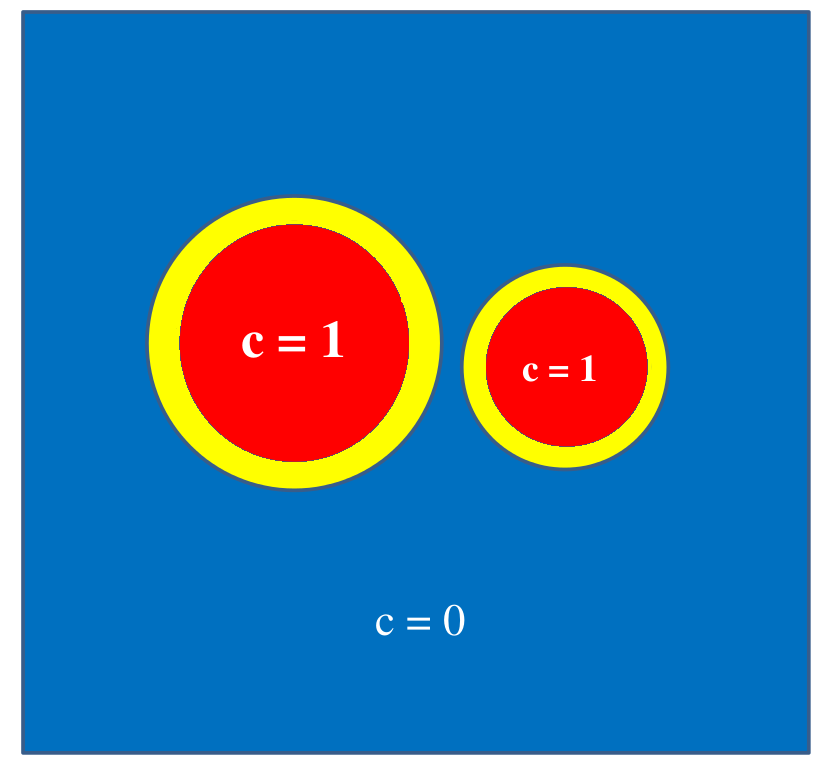
\includegraphics[scale=0.5]{Figure3}
\end{figure}
  
\subsection{Quantitative Two Phase Polynomial Free Energy Function}
Because of their similarities with double-well free energy function in predicting the growth and merging of voids/bubbles \cite{8}, polynomial free energy functions can be used to represent the bulk free energy term f(c,T) in equation (2).The polynomial function of orders 6 or 8 is defined as:
%%\begin{equation}
%%f = 128 \times W \sum_{m=1} ^{8} A_m c^m (8th order)
%%\end{equation}
%%\begin{equation}
%%f = 64 \times W \sum_{m=1} ^{6} A_m c^m 
%%\end{equation}
\begin{equation}
f = 2^{n} \times W \sum_{m=1} ^{n} A_m c^m 
\end{equation}
with n = 6 or 8.
In equation (3), W is the bubble barrier height. Denoting the equilibrium concentration between the gas bubble and molten metal as $c_{eq}$, the coefficients ($A_m$) for sixth order polynomial function in the above equation are expressed as:
$
A_1 =  \frac{3}{2} \left(c_{eq} ^2 + c_{eq} \right); 
A_2 = - \frac{9}{2} \left(c_{eq} ^2 + \frac{9}{2} c_{eq} + \frac{3}{4}\right);
A_3 = 6 c_{eq} ^2 - 6 c_{eq} - \frac{7}{2}; 
A_4 = -3.0 c_{eq} ^2 + 3.0 c_{eq} + \frac{27}{4};
A_5 = -6;
A_6 =  2. 
$ Similarly, these coefficients for 8th order polynomial functions are:
$
A_1 = - \frac{3}{2} \left(c_{eq} ^2 + c_{eq} \right); 
A_2 =  \frac{15}{2} \left(c_{eq} ^2 + 9 c_{eq} + \frac{3}{4}\right);
A_3 = -20 c_{eq} ^2 - 30 c_{eq} - \frac{11}{2}; 
A_4 = 30 c_{eq} ^2 + 60 c_{eq} + \frac{75}{4};
A_5 = 24 c_{eq} ^2 - 72 c_{eq} -36;
A_6 =  8c_{eq} ^2 + 48 c_{eq} +40; 
A_7 = \frac{96}{7} c_{eq} - 24; 
A_8 = 6.
$
The quantitative expressions for the phase field model parameters ( equilibrium concentration, gradient energy coefficient, barrier height, and  mobility,) as required by the polynomial free energies are obtained in accordance to the derivation given in \cite{12}, \cite{13}.The equilibrium concentration has been utilized to define the locations of the wells in the polynomial free energy function. Mathematically, it is defined as:
\begin{equation}
c_{eq} = e^{(- \frac{E_f}{k_{b}T})}
\end{equation}
In the above expression, $E_f$ is the enthalpy of formation of vacancy in tin at the given temperature T and $k_b$ is the Boltzmann constan$\mu$m t.Thus, the equilibrium concentration is lowered as the temperature increases.
The two model parameters- gradient energy coefficient ($k_{g}$) and barrier height (W) is expressed as functions of surface energy of tin ($\gamma$) and interface width ($l_i$) for the bubble as:
\begin{equation}
k_{g} = \frac{\gamma l_i}{B_n}
\end{equation} 
\begin{equation}
W = \frac{\gamma}{2B_{n}l_i}
\end{equation}
The variable $B_n$ in equations (5) and (6), is a function of $c_{eq}$, and is defined as following for the given polynomial order n:
\begin{equation}
B_n =2^{\frac{n}{2}} \int _{0} ^{1} \sqrt{\sum _{m=0} ^{n} A _{m} ^{n} c _{eq} ^{\frac{m}{2}} dc_{eq}}
\end{equation} 
For $c_{eq} << 1$, $B_n$ can be assumed to be a constant and has calculated values of $B_{6}$=0.78 and $B_{8}$=0.83551.
Finally, considering that the bubbles interaction phenomenon in liquid tin medium will follow the Fick's law of diffusion \cite{10}; the mobility for the polynomial free energy can be written as:
\begin{equation}
M = \frac{B_{n} \times D \times l_i}{512 \times A _{2} ^{6} \times \gamma}
\end{equation}
The diffusion of vacancies in tin material can be explained by the concept of self-diffusion coefficient, which is expressed in the following mathematical form:
\begin{equation}
D = D_{o} \times e ^{(\frac{-E_{m}}{k_{b}T})}
\end{equation}
where, $E_m$ is the energy of vacancy motion in tin \cite{10}.

\subsection{Temperature in Liquid Tin}
For the solder material having physical dimensions in the scale of micrometers, Biot number is very small ($Bi << 1$) and conduction is the dominant mode of heat transfer. Hence, the temperature variation of the solder medium for steady state assumptions can be represented by the following equation.
%\begin{equation}
%\rho C_{p}\frac{\partial T}{\partial t} = k_{th} \triangledown T
%\end{equation}
%wherein, $\rho$, $C_p$ and $k_{th}$ are the density, heat capacity and thermal conductivity of tin material. For steady state, equation (10) can be reduced to the given structure:
\begin{equation}
k_{th} \triangledown T = 0
\end{equation}
wherein, $k_{th}$ is the thermal conductivity of liquid tin.
For the purpose of numerical ease, the above steady state heat conduction equation is solved with a linearly time-varying temperature boundary conditions readily available from the experimental data (section 2).In order words, the change in temperature of the solder medium with time, can be accounted for by supplying time-varying experimental temperatures values  at the four boundaries of the square domain. 
 

\subsection{Implementation of the Phase Field Model}
\subsubsection{Initial Size and Positions of Bubbles}
Three bubbles of initial radii 7 $\mu$m, 9 $\mu$m and 12 $\mu$m were defined within the square domain of size 150 $\mu$m $\times$ 150 $\mu$m.In order to get a comparative analysis of experimental bubble interactions, the bubble with the largest initial diameter was positioned at the middle with the smallest at its left and the intermediate at the right side (Figure 4). The initial distance between the smallest and the largest bubble is kept as 1 $\mu$m whereas its value is around 5 $\mu$m for the pair of largest and the intermediate bubble.
\begin{figure}
\caption{Initial condition in numerical model for sizes and positions of the bubbles}
\centering
  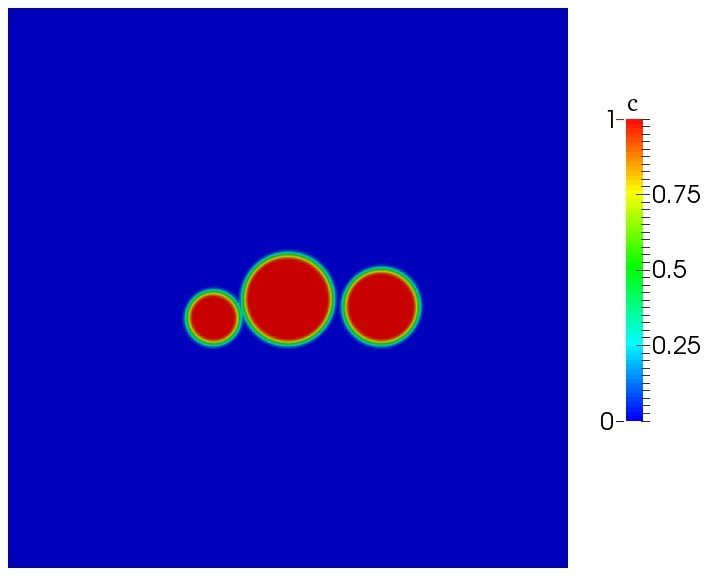
\includegraphics[scale=0.3]{Figure4}
\end{figure}
\subsubsection{Numerical Implementation}
Equation (1) coupled with the steady state heat conduction equation- Equation (10), is solved through finite element method using MOOSE software ( \cite{14}, \cite{15}, \cite{16}, \citep{17}).As mentioned early, time varying temperature values have been used as dirichlet boundary conditions at the four boundaries of the domain to indicate the temperature change of the domain.The material parameters for the phase field equation and the heat conduction equations have been highlighted in Table 1.
\subsection*{Table 1: Parameters for the Materials Properties}
\begin{tabular}{|c|c|c|c|}
\hline 
Parameters & Values & Units & Remarks  \\ 
\hline 
$E _f$ & 0.511 & ev & $\cite{18}$ \\ 
\hline 
$E _m$  & 0.681 & ev  & $\cite{18}$ \\ 
\hline 
$D_o$ & $3.28 \times 10 ^{-4}$ & $ m^{2}/s $ & $\cite{19}$, $\citep{20}$ \\ 
\hline 
$k_{th}$ & 31.63 & $W/(m K)$ & $\citep{21}$ \\ 
\hline
$\gamma$ & 0.56 & $J/m^{2}$ & $\citep{2}$,$\citep{22}$ \\ 
\hline
$\frac{d\gamma}{dT}$ & $-2.0 \times 10 ^{-4}$ & $J/(m^{2} K)$ & $\citep{22}$,$\citep{23}$ \\ 
\hline
\end{tabular} 

\subsection*{•}
A function is utilized to switch the thermal conductivity values in between the tin and the bubble.The temperature coefficient of surface energy is utilized to define the decrease of surface tension with temperature rise.The total time for the simulation has been taken as 60 s.The length and time scales have been defined as 1 nm and 1 ms respectively. The time step size of the simulation has been considered as 1 s. In order to assess the role of diffuse-interface width ($l_i$) as well as its relation to grid spacing ($\Delta x = \Delta y$ = 0.75 $\mu m$) in the results of numerical simulation ($\citep{12}, \citep{13}$); the conditions listed in Table 2, have been employed in the phase field model.
\subsection*{Table 2:Values of interface width and grid spacing used in numerical simulation}
\begin{tabular}{|c|c|c|c|c|}
\hline
Model Type & Polynomial Order (n) &  $l_i (\mu m)$ & $\frac{l_i}{\Delta x}$ & $k_{g}$ ($\times 10^{6}$) \\
\hline
I & 6 &  3.3 & 4.4 & 2.37 \\
\hline
II & 6 & 5 & 6.67 & 3.6 \\
\hline
III & 8 & 3.3 & 4.4 & 2.21 \\
\hline
IV & 8  & 5 & 6.67 & 3.35 \\
\hline
\end{tabular}
\subsection*{•}
 Denoting $r_c$ as the radius of curvature of the smallest bubble, the numerical convergence becomes more difficult for smaller $\frac{r_c}{l_i•}$ values $\citep{24}$. Because of the convergence issue, the greater of the two $l_i$ values was limited to 5 $\mu m$. 

\section{Results and Discussion}

\subsection{Numerical Results}
As already mentioned in table 2, the bubbles for two different interval width and two different orders of polynomial functions, were modeled with the $\dot P_{flux}$ values of 0, 2.0 $\times 10 ^{-4}$ and 5.0 $\times 10 ^{-4}$ $c/s$. The final size of the elliptical bubble for the simulation time of 60 s have been plotted in bar chart in Figure 7. It is observed from the figure that models I and IV have yielded the final size (t=60 s) of the merged bubble nearly equal to the experimental value when $P_{flux} = 2.0 \times 10 ^{-4}$.   It is interesting to note here that the results of the numerical simulation validated with the experimental figures, could be used to assess the production or release rate of  gaseous particle from the heated flux at elevated temperatures.
\begin{figure}
\caption{Bar chart showing the major axis and minor axis of the final elliptical bubble (at t=60 s) of the numerical model(types I, II, III and IV outlined in table 2) for different values of source gas ($P_{flux}$). Types I ($l_{i}=3.3 \mu m$) and II($l_{i}=5 \mu m$) correspond to polynomial function of order 6 whereas III($l_{i}=3.3 \mu m$) and IV($l_{i}=5 \mu m$) use the order 8 polynomial function.}
\centering
   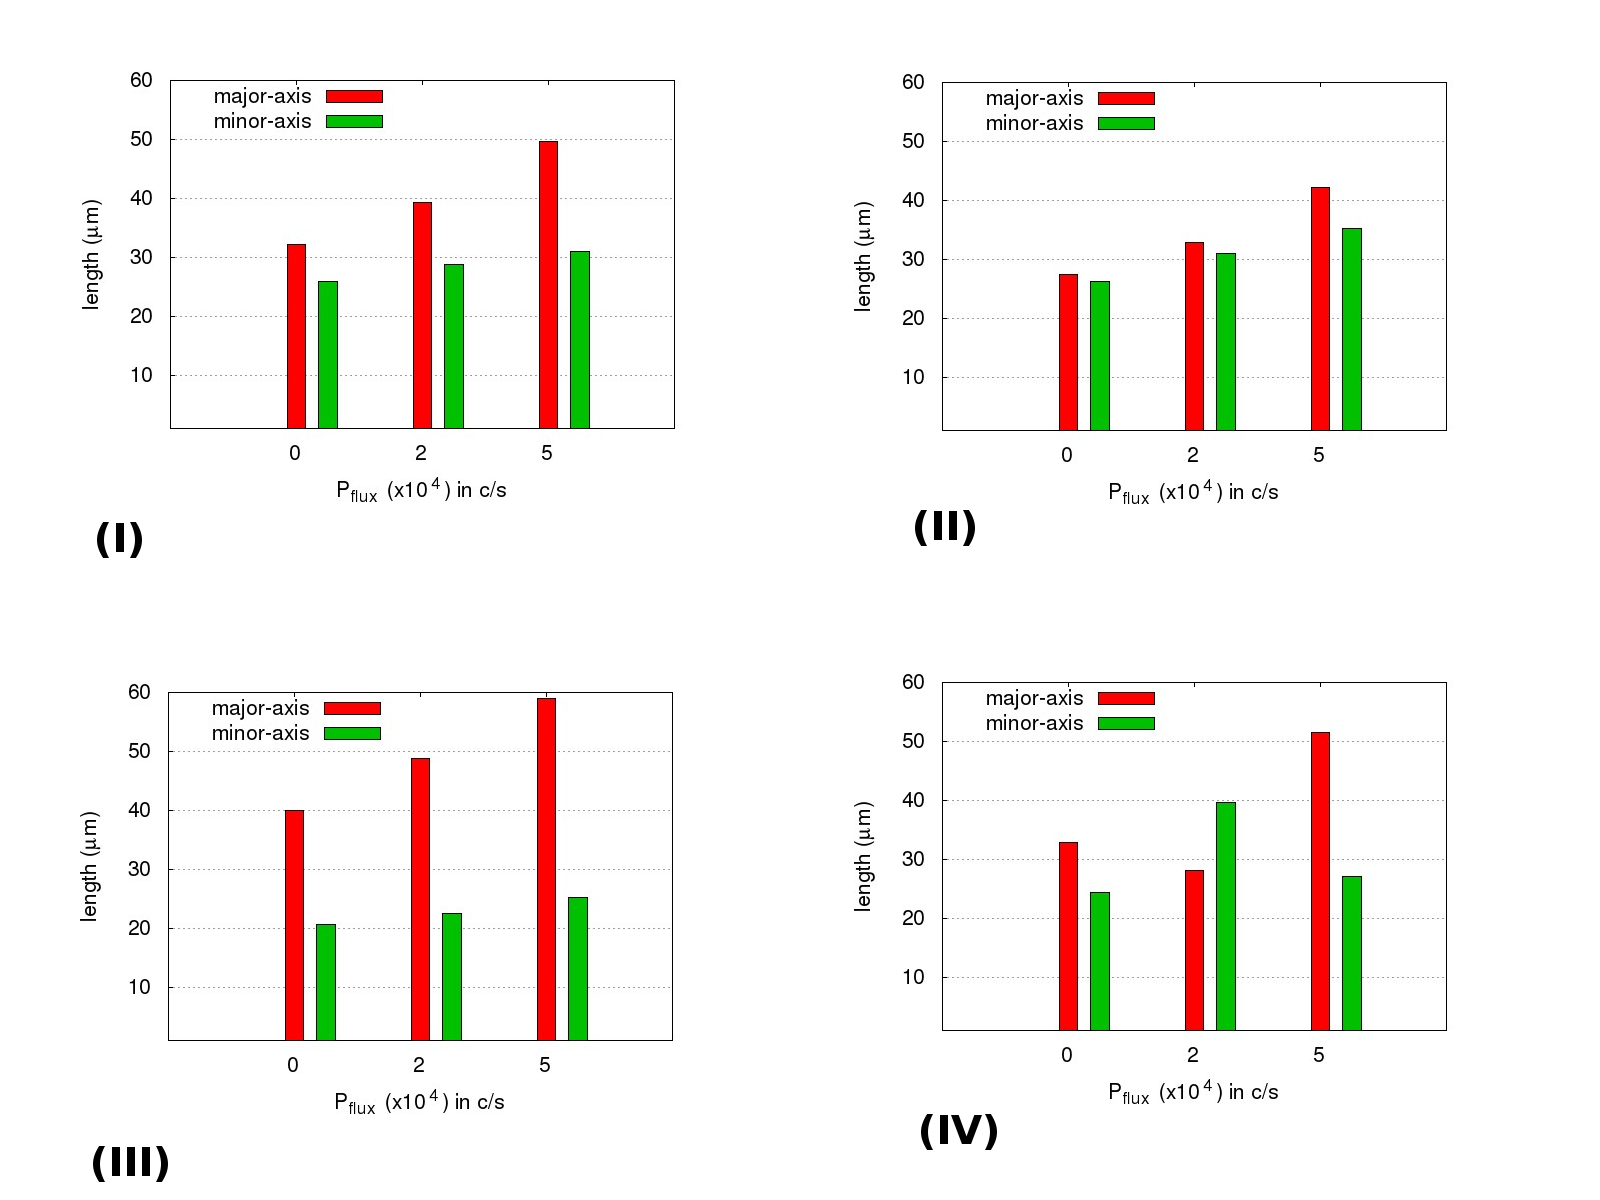
\includegraphics[scale=0.25]{Bubble60}
\end{figure}  
%\subsubsection{Roles of $l_{i}$ and $k_{g}$}
\subsubsection*{•}
Figure 8 and 9 represent the bubble profiles at different point of time for the numerical models I and IV, and the nomenclature of the bubbles is considered to be same as that of the experimental bubbles. The overall trend of the growth, attachment and annexation phenomena as shown by the numerical simulation is in satisfactory agreement with the experimental results. Notable in the numerical model is the observation of ostwald ripening phenomenon \citep{1}, \citep{10}. Provided that A (smallest) and B (largest) bubbles are in surface contact, it has been shown in the figures that gas flux from bubble A is driven into the bubble B during annexation. Similarly, the smaller bubble C is driven into the another end surface of bubble B. In general,for adjacent bubble 1 and bubble 2 of radii $R_1$ and $R_2$ respectively, such that $R_1 > R_2$, the pressures in the bubble 2 would be greater than that in bubble 1in accordance to the following relation of the Gibbs-Thomson effect:
\begin{equation}
ln(\frac{p_2}{p_1})= k (\frac{1}{R_2}-\frac{1}{R_1})
\end{equation} 
Thus, because of this pressure differences in the three bubbles, there will be a disbalance of mechanical equilbrium that will eventually lead to their merging. Hence, bubble A and bubble C, each of smaller radius than bubble B, would be driven into bubble B, inorder to give a final bubble D. 
\subparagraph*{•}
\begin{figure}
\caption{Profiles of the annexing bubbles for 6th order polynomial functions and $k_{g}= 2.37 \times 10 ^{-6}$, at (a) t=0, (b) t =5, (c) t=10, (d) t=15, (e) t=30, (f) t=40, (g) t=50, and (h)t=60 s.}
\centering
	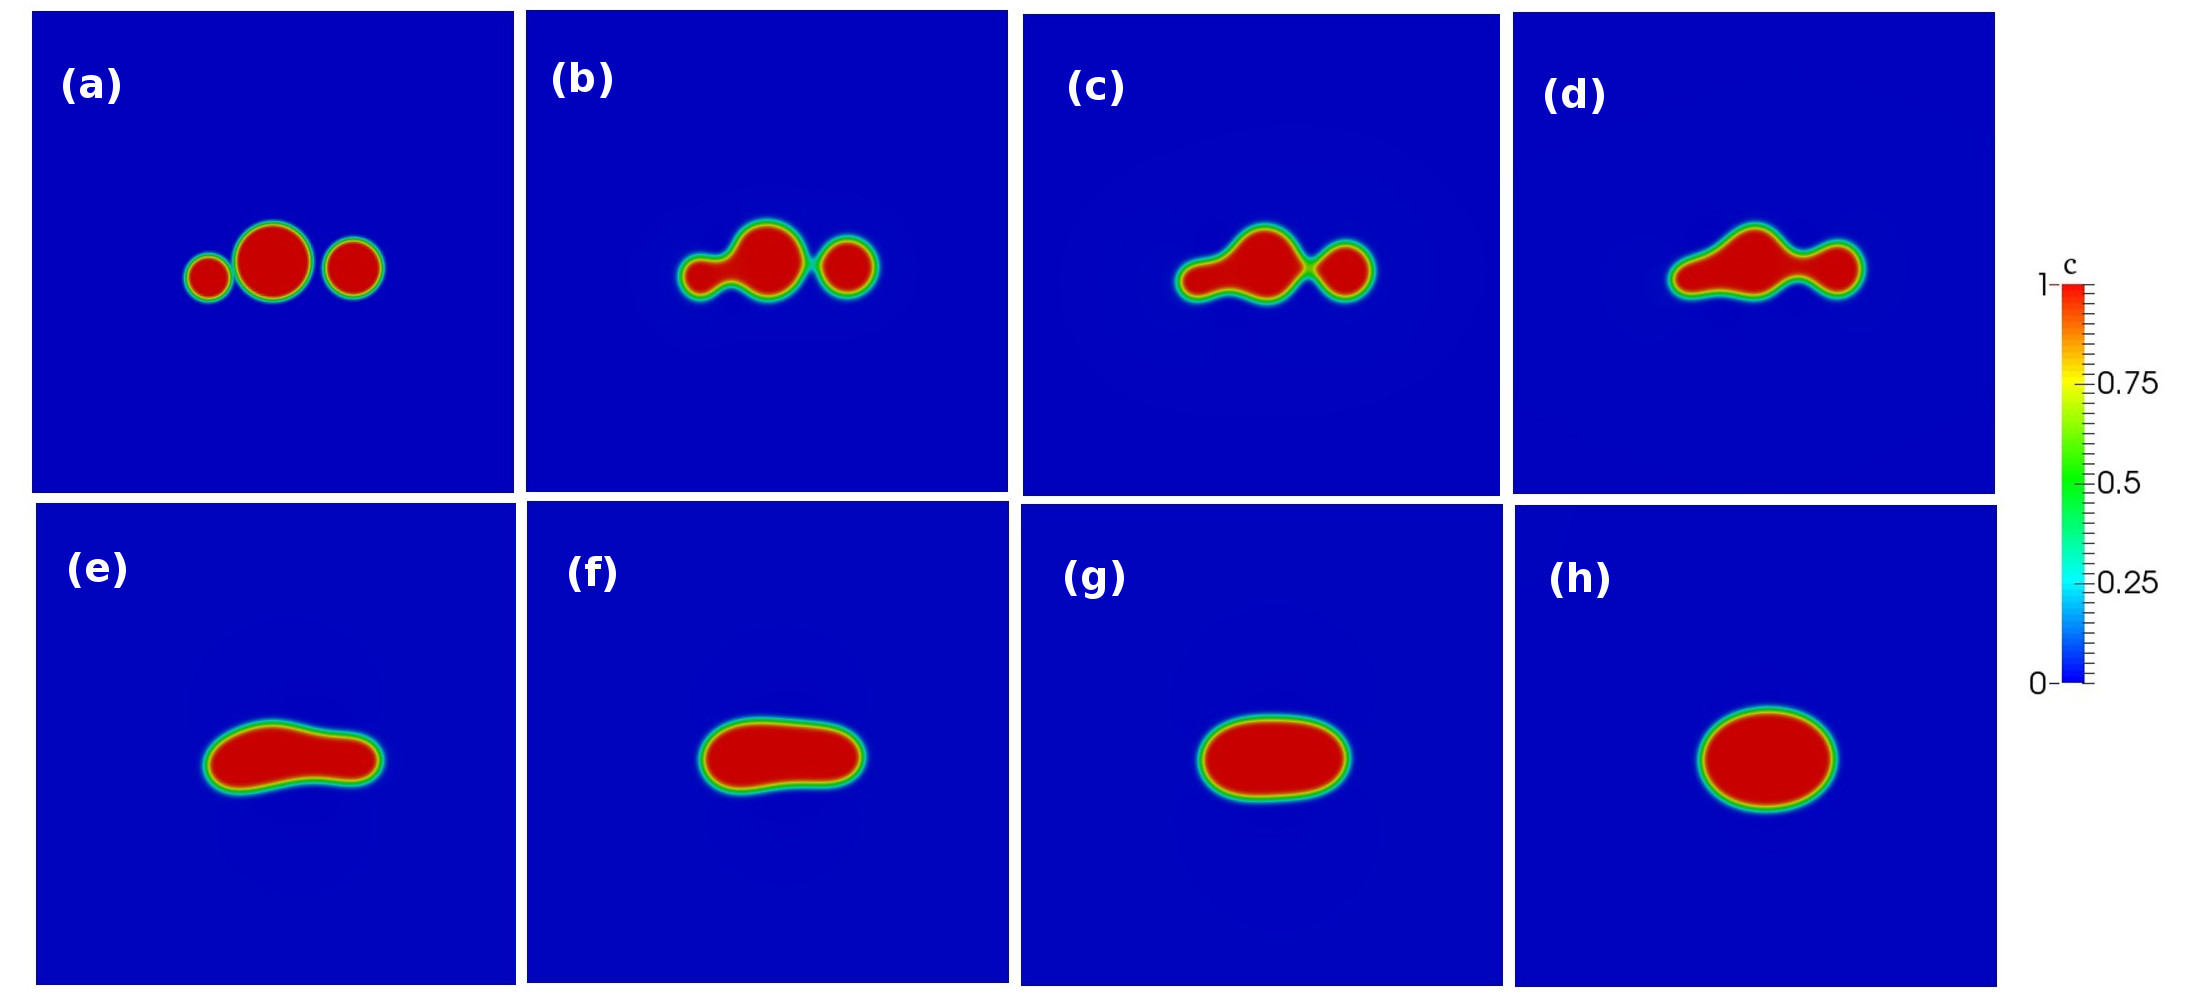
\includegraphics[scale=0.175]{poly6iw33pg2104}
\end{figure}
\subsubsection{Roles of interface width and gradient energy coefficient in the accuracy of shape description}
The model IV represented by figure 9 has larger $\frac{l_{i}}{\delta x}$ and subsequently greater gradient energy coefficient ($k_{g}$) than model I corresponding to figure 8.Though the final size of the bubble is obtained to have similar size in both types, the shape description of the interacting bubbles and the annexed bubble during the entire simulation is not exactly the same. It is evident from these figures that model IV, with greater $\frac{l_{i}}{\Delta x}$ and  $k_{g}$ values, can express the curvature changes in a more pronounced way thus suggesting that larger interval width is more favorable for the shape description of the curves in a domain of given grid dimension ($\citep{12}, \citep{13}$). For example, at t = 5 s, while comparing between figures 8 and 9, it could be observed that larger interval width and subsequently, larger gradient energy coefficient provides pronounced curvature tracking of the smallest bubble at the left when it is interacting with the largest bubble. In the same way, the curvature description of the intermediate bubble at the far right is more distinct in figure 9 as compared to figure 8 at t=15 s.  Also, the larger value of interfacial gradient energy (greater $l_{i}$ and smaller $B_n$ is responsible for the quicker attainment in the spherical shape for the bubble. Thus, the interface width used for Polynomial function of order 8 should be greater than that of 6th order model, as the latter has the higher magnitude of $B_n$.As shown in figure 10, the bubble for polynomial function order 8 having $k_g$ value equal to $2.21 \times 10 ^{-6}$ i.e. the lowest among all the four models, has the greatest eccentricity value at t = 60 s. Model II with 6th order polynomial function and $k_g = 3.6 \times 10 ^{-6}$ (greatest among all the models), has the bubble attain a nearly spherical shape by the time of 60 s (figure 11). This results can be used to explain the role of magnitude of the material property -surface energy in the change rate of geometry of the bubble. In accordance to equation (5), $k_g$ is directly proportional to surface tension and thus  it could be inferred that materials with greater magnitude of surface energy values will have their bubbles attain spherical profile at a quicker rate. 
\begin{figure}
\caption{Profiles of the annexing bubbles for 8th order polynomial functions and $k_{g}= 3.35 \times 10 ^{-6}$, at (a) t=0, (b) t =5, (c) t=10, (d) t=15, (e) t=30, (f) t=40, (g) t=50, and (h)t=60 s.}
\centering
	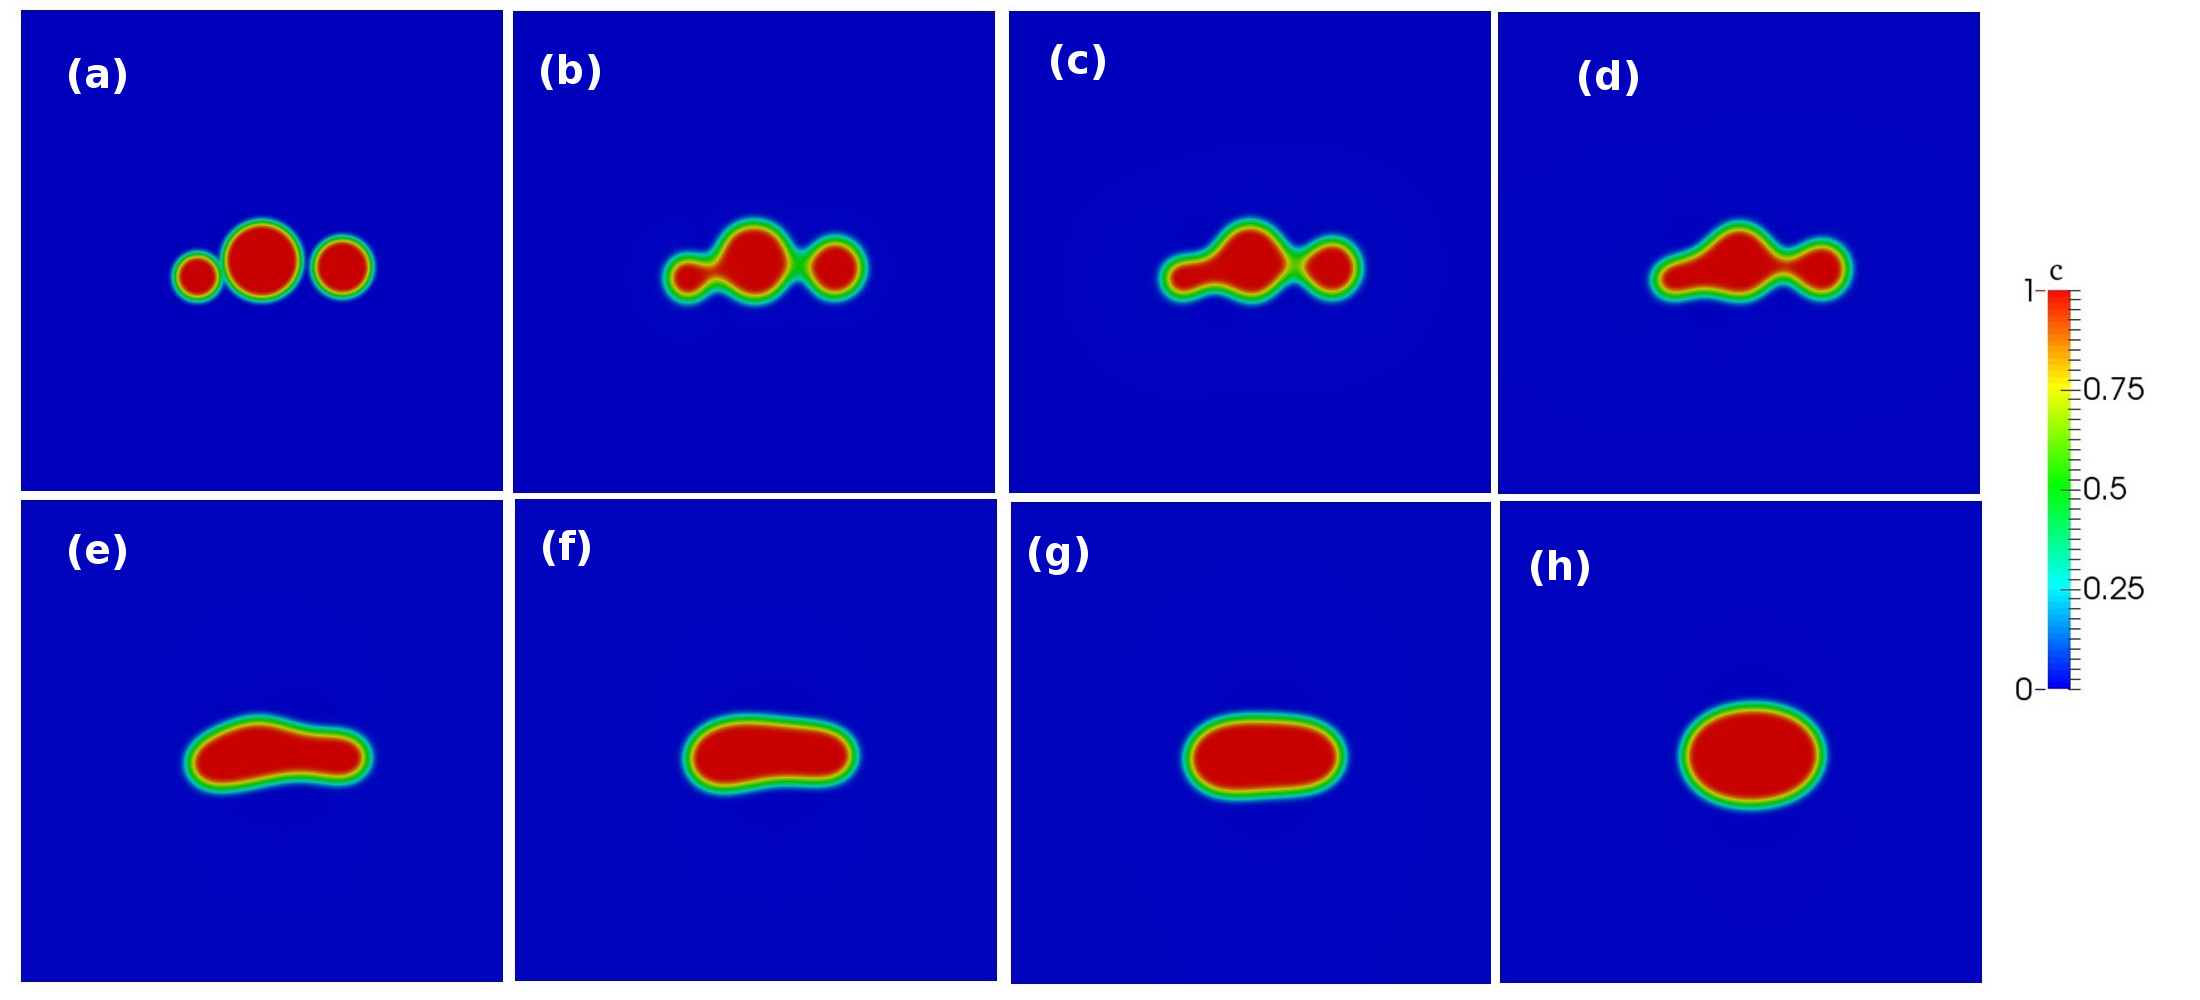
\includegraphics[scale=0.175]{poly8iw5pg2104}
\end{figure}
\subsubsection{Physical properties of material in the numerical model}
The energy of motion of vacancies, surface energy, diffusion coefficient and the thermal conductivity of the materials can largely affect the kinetics of bubble annexation. The lower $E_m$ and higher D values are associated with the faster merging of solder bubbles in accordance to equations (1), (9) and (10).  Significantly, temperature increment causes the increase in the diffusion coefficient and temperature can be considered as the important parameter in the bubble annexation phenomenon.Similarly, the growth of bubbles in the temperature field will be accelerated for materials with higher thermal conductivity. As mentioned in section 4.2.1, surface energy is associated with the attainment rate of geometrical profile of the void or bubbles. The effect of these material parameters could be numerically evaluated through the phase field model. Thus, the phase field analysis can be an important material design method for design of solder materials in connection to void control.
\begin{figure}
\caption{Elliptical bubble corresponding to model IV(8th order Polynomial Function and $k_g = 2.21 \times 10 ^{-6}$) has the greatest eccentricity among all the models at t=60 s for a given value of $P_{flux}$.}
\centering
	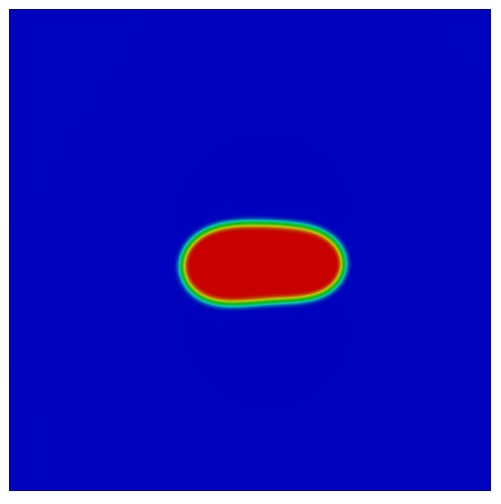
\includegraphics[scale=0.5]{poly8iw33t60}
\end{figure}

\begin{figure}
\caption{Elliptical bubble corresponding to model II(6th order Polynomial Function and $k_g = 3.6 \times 10 ^{-6}$) has the lowest eccentricity among all the models at t=60 s for a given value of $P_{flux}$.}
\centering
	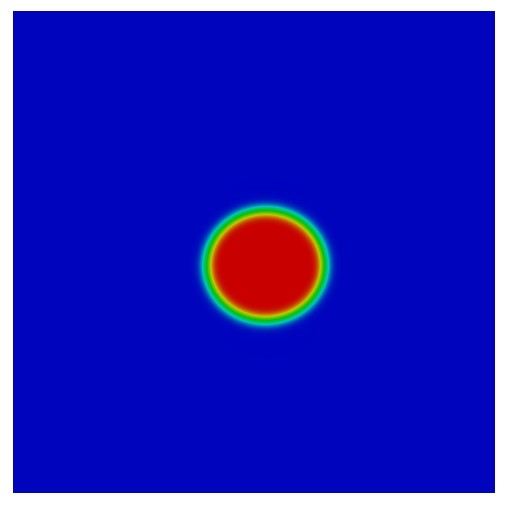
\includegraphics[scale=0.5]{poly6iw5t60}
\end{figure}

%% The Appendices part is started with the command \appendix;
%% appendix sections are then done as normal sections
%% \appendix

%% \section{}
%% \label{}

%% If you have bibdatabase file and want bibtex to generate the
%% bibitems, please use
%%
%%  \bibliographystyle{elsarticle-num} 
%%  \bibliography{<your bibdatabase>}




%% else use the following coding to input the bibitems directly in the
%% TeX file.

\section*{Reference}
%%\label{}

\begin{thebibliography}{00}

%% \bibitem{label}
%% Text of bibliographic item
\bibitem{1} L. Qu, H.T. Ma, H.J. Zhao, A. Kunwar, N. Zhao, Appl. Surf. Sci. 305 (2014) 133.

\bibitem{2} A. Kunwar, H. Ma, J. Sun, S. Li, J. Liu, Met. Mater. Int. 21 (2015).

\bibitem{3} S. Lee, H.M. Zhou, D.F. Baldwin, Model. Simul. Mater. Sci. Eng. 18 (2010) 065005.

\bibitem{4} D.N. Bhate, A. Kumar, A.F. Bower, J. Appl. Phys. 87 (2000) 1712.

\bibitem{5} M. Mahadevan, R.M. Bradley, Phys. D Nonlinear Phenom. 126 (1999) 201.

\bibitem{6} J.W. Cahn, J.E. Hilliard, J. Chem. Phys. 28 (1958) 258.

\bibitem{7} P.C. Millett, A. El-Azab, S. Rokkam, M. Tonks, D. Wolf, Comput. Mater. Sci. 50 (2011) 949.

\bibitem{8} P.C. Millett, A. El-Azab, D. Wolf, Comput. Mater. Sci. 50 (2011) 960.

\bibitem{9} S. Hu, C.H. Henager, H.L. Heinisch, M. Stan, M.I. Baskes, S.M. Valone, J. Nucl. Mater. 392 (2009) 292.

\bibitem{10} M.R. Tonks, S.B. Biner, P.C. Millett, D. A. Andersson, in:, Int. Conf. Math. Comput. Methods Appl. to Nucl. Sci. Eng. (M \& C 2013), American Nuclear Society, Sun Valley, Idaho,USA, 2013.

\bibitem{11} L. Zhang, M.R. Tonks, P.C. Millett, Y. Zhang, K. Chockalingam, B. Biner, Comput. Mater. Sci. 56 (2012) 161. 

\bibitem{12} N. Moelans, B. Blanpain, P. Wollants, Phys. Rev. Lett. 101 (2008) 1.

\bibitem{13} N. Moelans, B. Blanpain, P. Wollants, Phys. Rev. B - Condens. Matter Mater. Phys. 78 (2008)

\bibitem{14} D. Gaston, C. Newman, G. Hansen, D. Lebrun-Grandié, Nucl. Eng. Des. 239 (2009) 1768.

\bibitem{15} M. Tonks, D. Gaston, C. Permann, P. Millett, G. Hansen, D. Wolf, Nucl. Eng. Des. 240 (2010) 2877.

\bibitem{16} M.R. Tonks, D. Gaston, P.C. Millett, D. Andrs, P. Talbot, Comput. Mater. Sci. 51 (2012) 20.

\bibitem{17} D.A. Knoll, D.E. Keyes, J. Comput. Phys. 193 (2004) 357.

\bibitem{18}  P.H. Sun, M. Ohring, J. Appl. Phys. 47 (1976) 478.

\bibitem{19} R.A. Swalin, C.H. Ma, J. Appl. Phys. 36 (1962) 3014.  

\bibitem{20} J.P. Foster, R.J. Reynik, Metall. Trans. 4 (1973) 207. 

\bibitem{21} M. V. Peralta-Martinez, W. A. Wakeham, Int. J. Thermophys. 22 (2001) 395.

\bibitem{22} Z.F. Yuan, K. Mukai, K. Takagi, M. Ohtaka, W.L. Huang, Q.S. Liu, J. Colloid Interface Sci. 254 (2002) 338. 

\bibitem{23} N. Eustathopoulos, B. Drevet, E. Ricci, J. Cryst. Growth 191 (1998) 268.

\bibitem{24} I.M. McKenna, M.P. Gururajan, P.W. Voorhees, J. Mater. Sci. 44 (2009) 2206. 

\end{thebibliography}
\end{document}